\section{Multivariable Integrals}

Abstractly, the processes of integration is:
(i) chop a region into easy to 
approximate pieces, (ii) approximate each tiny piece, (iii) add together
the approximations, and (iv) take a limit as the size of each piece tends to zero\footnote{
If your approximations get better and better as the size of each piece shrinks,
the whole process works.  This isn't the case for all objects, but conditions like
differentiability and piecewise smooth are often sufficient.  It's annoying
to specify exactly what is needed over and over again, so sometimes we just say
an object is ``nice.''}.
 Thus far, the domain of this procedure---the
thing we chop into tiny pieces---has been a line or curve.  We will now consider
integrating over multi-dimensional domains.

We will start by finding the area of a region in the plane.
Let $\mathcal R\subseteq \R^2$ be the region below the line $y=1$ and above the
curve $y=x^2$.  We wish to find the area of $\mathcal R$.


\begin{center}
	\begin{tikzpicture}

		\begin{axis}[
		    anchor=origin,
		    set layers=standard,
		    disabledatascaling,
		    xmin=-2,xmax=2,
		    ymin=-1,ymax=2,
		    x=1.3cm,y=1.3cm,
		    grid=both,
		    grid style={line width=.1pt, draw=gray!10},
		    %major grid style={line width=.2pt,draw=gray!50},
		    axis lines=middle,
		    minor tick num=0,
		    enlargelimits={abs=0.5},
		    axis line style={latex-latex},
		    ticklabel style={font=\tiny,fill=white},
		    xlabel style={at={(ticklabel* cs:1)},anchor=north west},
		    ylabel style={at={(ticklabel* cs:1)},anchor=south west}
		]

	    	\addplot[name path=f,no marks,mypink,thick,domain=-1:1, samples=25, draw=none] ({x},{x*x});
	    	\addplot[no marks,mypink,thick,domain=-2:2, samples=25,smooth] ({x},{x*x});
	    	\addplot[name path=g, no marks,green!50!black,thick,domain=-3:3, samples=2] ({x},{1});
		\addplot [thick, color=blue, fill=blue, fill opacity=0.05] fill between [of=f and g, split];
		\draw (0,.3) node[above right] {$\mathcal R$};
		\draw [mypink,fill] (1.2,1)  node [above right] {$y=x^2$};
		\draw [green!50!black,fill] (-2,1)  node [below right] {$y=1$};

		\end{axis}
	\end{tikzpicture}
\end{center}

Using the usual calculus strategy, we will chop $\mathcal R$ up into little rectangles
of width $\Delta x$ and height $\Delta y$.  Then
\[
	\text{area of }\mathcal R \quad\approx \sum_{\text{tiny rectangles}}\text{area of tiny rectangle}
\]
and
\[
	\text{area of }\mathcal R =\lim_{\Delta x,\Delta y\to 0} \sum_{\text{tiny rectangles}}\text{area of tiny rectangle}.
\]

\begin{center}
	\begin{tikzpicture}[x=2cm,y=2cm,
]

\begin{scope}[	spy using outlines={circle, lens={scale=4}, size=3cm, connect spies}]
		\coordinate (A) at (.3,.15*4);
		\coordinate (B) at (.4,.15*5);
		\fill[gray,opacity=.5] (A) rectangle (B);


		\begin{axis}[
		    anchor=origin,
		    set layers=standard,
		    disabledatascaling,
		    xmin=-1,xmax=1,
		    ymin=0,ymax=1,
		    x=2cm,y=2cm,
		    grid=both,
		    grid style={line width=.1pt, draw=gray!10},
		    %major grid style={line width=.2pt,draw=gray!50},
		    axis lines=middle,
		    minor tick num=0,
		    enlargelimits={abs=0.4},
		    axis line style={latex-latex},
		    ticklabel style={font=\tiny,fill=white},
		    xlabel style={at={(ticklabel* cs:1)},anchor=north west},
		    ylabel style={at={(ticklabel* cs:1)},anchor=south west}
		]

	    	\addplot[name path=f,no marks,mypink,thick,domain=-1:1, samples=25, draw=none] ({x},{x*x});
	    	\addplot[no marks,mypink,thick,domain=-2:2, samples=25,smooth] ({x},{x*x});
	    	\addplot[name path=g, no marks,green!50!black,thick,domain=-3:3, samples=2] ({x},{1});
		\addplot [thick, color=blue, fill=blue, fill opacity=0.05] fill between [of=f and g, split];

		\end{axis}
			\foreach \x in {-1,-.9,...,1} {
				\draw ($(\x,1)$) -- ($(\x,\x*\x)$);
			}
			\foreach \y in {0,.15,...,1} {
				\draw ({-\y^.5,\y}) -- ({\y^.5,\y});
			}


		\spy [blue] on ($.5*(A)+.5*(B)$)
             in node (a) at (3,1);


\end{scope}
	\coordinate (L) at ($(a.center) - (.2,.3)$);
\coordinate (R) at ($(a.center) - (-.2,.3)$);
\coordinate (T) at ($(a.center) + (.2,.3)$);
		\draw[decoration={brace, mirror}, decorate, mypink] ($(R)+(.03,0)$) -- ($(T)+(.03,0)$) node[midway, right] {$\Delta y$};
\draw[decoration={brace, mirror}, decorate,mypink] ($(L)-(0,.03)$) -- ($(R)-(0,.03)$) node[midway, below] {$\Delta x$};

		
	\end{tikzpicture}
\end{center}


Using integral notation, we would write
\[
	\text{area of }\mathcal R=\int_{\mathcal R} \d A.
\]
Here, $\d A$ represents a ``tiny area,'' the subscript $\mathcal R$ represents the region of integration,
and the integral sign means we're adding things up.  In this case, we're finding area, so $\d A=1\d A$ is
exactly what we're adding up.  In other situations, we'll be adding up more complicated quantities.

This is all well and good, but how do we actually \emph{find} the area?  To do this, we'll
need to convert $\int_{\mathcal R}\d A$ into a more traditional-looking integral---one that we
know how to evaluate.

Let's write down our sum more carefully.  We need to sum over all tiny rectangles that fit inside
$\mathcal R$.  To do so, we can take a systematic approach: sum all the rectangles
in a column first and then sum up all the columns.  The lower left corner of all 
rectangles in a single column share a common $x$-coordinate.  Consider
the column with lower left corner at $(x_0,y_0)$.  Counting, we see there
are approximately $(1-x_0^2)/\Delta y$ rectangles in this column.  Further, there are approximately
$2/\Delta x$ columns.  Therefore,
\[
	\text{area of }\mathcal R\approx 
	\sum_{i=1}^{2/\Delta x}\quad\sum_{j=1}^{(1-(i\Delta x)^2)/\Delta y} \Delta y\Delta x.
\]
That sum is really hard to parse, so we'll write it another way.
\[
	\text{area of }\mathcal R\approx
	\sum_{x_0=-1,\,-1+\Delta x,\ldots,1}
	\quad
	\sum_{y_0=x_0^2,\,x_0^2+\Delta y,\ldots,1}
	\Delta y\Delta x.
\]
This is still hard to read, but it's looking more like an integral.  The inner sum
is adding up things from $y_0=x_0^2$ to $y_0=1$ and the outer sum is adding up
things from $x_0=-1$ to $x_0=1$.  After taking the limit
as $\Delta x,\Delta y\to 0$, we may rewrite this as an
integral, giving
\begin{equation}
	\label{EQITERATEDINT}
	\text{area of }\mathcal R\quad
	=\quad
	\int_{\mathcal R}\d A \quad =\quad \int_{x=-1}^{x=1}\int_{y=x^2}^{y=1} \d y\d x.
\end{equation}
Now, we should take a moment to make sure we understand what we've just written.  The
right side of Equation \eqref{EQITERATEDINT} is an \emph{iterated integral}\index{iterated integral}.
That is,
\[
	\int_{x=-1}^{x=1}\int_{y=x^2}^{y=1} \d y\d x
	\quad 
	=
	\quad \int_{x=-1}^{x=1}\left(\int_{y=x^2}^{y=1} \d y\right)\d x
\]
and so the integral with respect to $y$ must be done \emph{before} the integral with respect to $x$.
To be clear, $\d y$ and $\d x$ are \emph{not} being multiplied.  However, $\Delta y$ and $\Delta x$ 
\emph{were} being multiplied in our sum expression.  What happened?  The answer is some slight of
hand.  We can write a more complete list of steps:\footnote{ Even still, we skipped steps.
In particular, we split up $\lim_{\Delta x,\Delta y\to 0}$ into two limits 
$\lim_{\Delta x\to 0}\lim_{\Delta y\to 0}$.  Then, we exchanged a limit and a sum.  These
steps require justification, but we won't trouble ourselves with that here.}
\[
	\lim_{\Delta x,\Delta y\to 0} \sum_{x_i}\sum_{y_i} \Delta y\Delta x
	=
	\lim_{\Delta x,\Delta y\to 0} \sum_{x_i}\left(\sum_{y_i} \Delta y\right)\Delta x
	=\int_{x=-1}^{x=1}\left(\int_{y=x^2}^{y=1} \d y\right)\d x.
\]

Now we can evaluate this iterated integral to conclude
\[
	\text{area of }\mathcal R
	\quad
	=\quad
	\int_{\mathcal R}\d A \quad=\quad 
	\int_{x=-1}^{x=1}\left(\int_{y=x^2}^{y=1} \d y\right)\d x \quad=\quad
	\tfrac{4}{3}.
\]
But, there was another way we could have divided up our original sum.  
We could have summed all tiny rectangles in a single row first and then 
added up all the row sums.
Using this approach, we see
\[
	\lim_{\Delta x,\Delta y\to 0} \sum_{y_i}\sum_{x_i} \Delta x\Delta y
	=
	\lim_{\Delta x,\Delta y\to 0} \sum_{y_i}\left(\sum_{x_i} \Delta x\right)\Delta y
	=\int_{y=0}^{y=1}\left(\int_{x=-\sqrt{y}}^{x=\sqrt{y}} \d x\right)\d y.
\]
Computing this integral, we again get $4/3$, as expected.

Note that when we swapped the order of the sums (and hence the order of the integrals)
the bounds changed.  This is worth considering carefully.

When we integrate with respect to $y$ and then $x$, it means that we first imagine
$x$ is fixed and we let $y$ vary between bounds (which may depend on the fixed $x$).
When we integrate with respect to $x$ first, the situation is reversed.  Geometrically,
it's easy to see why our bounds change.

\begin{center}
	\begin{tikzpicture}

		\begin{axis}[
			name=plot0,
			anchor=origin,
		    xmin=-1,xmax=1,
		    ymin=0,ymax=1,
		    x=2cm,y=2cm,
		    grid=none,
			hide axis,
		]


		\addplot[domain=-1:1, smooth, draw=black, fill opacity=0.05, fill=blue] (x,x^2) -- cycle;

		\draw[fill=mypink,draw=none] (-.7,.49) node (A) {} rectangle (.7,.51) node (B) {};
		\draw (-.7,-.2) node (A1) {};
		\draw(.7,-.2) node (B1) {};

		\draw (-1,1) node (C) {} (-1,0) node (C2) {};



		\end{axis}

		\draw[densely dashed] (A) -- (A1) (B) -- (B1);
		\draw[decoration={brace, mirror, raise=0cm}, decorate, thick] (A1) -- (B1) node[midway, below] {$-\sqrt{y}\leq x \leq \sqrt{y}$};
		\draw[decoration={brace, mirror, raise=0.1cm}, decorate, thick] (C) -- (C2) node[midway, left, xshift=-.2cm] {$0\leq y \leq 1$};

		\begin{axis}[
			name=plot1,
			xshift=1cm,
			at=(plot0.right of south east),
		    xmin=-1,xmax=1,
		    ymin=0,ymax=1,
		    x=2cm,y=2cm,
		    grid=none,
			hide axis,
		]

		\addplot[domain=-1:1, smooth, draw=black, fill opacity=0.05, fill=blue] (x,x^2) -- cycle;

		\draw[fill=mypink,draw=none] (.3,.09) node (A) {} rectangle (.32,1) node (B) {};
		\draw (1.2,.09) node (A1) {};
		\draw(1.2,1) node (B1) {};

		\draw (-1,0) node (C) {} (1,0) node (C2) {};
		\end{axis}

		\draw[densely dashed] (A) -- (A1) (B) -- (B1);
		\draw[decoration={brace, mirror, raise=0cm}, decorate, thick] (A1) -- (B1) node[midway, right,xshift=.1cm] {$x^2\leq y \leq 1$};
		\draw[decoration={brace, mirror, raise=0.41cm}, decorate, thick] (C) -- (C2) node[midway, below, yshift=-.41cm] {$-1\leq x \leq 1$};
	\end{tikzpicture}
\end{center}

However, there's also an algebraic argument for why our bounds change.
Suppose $(x,y)\in\mathcal R$.  Then $-1\leq x\leq 1$ and $x^2\leq y\leq 1$.  These were the
bounds we used adding up along columns first.  However, we also know that $0\leq y\leq 1$
and $-\sqrt{x}\leq y\leq \sqrt{x}$, which gives the bounds when adding up
along rows first.  These two system of inequalities don't contradict each
other; they contain the exact same information.  The difference is in
which coordinates you can verify without the others.

Given $-1\leq x\leq 1$ and $x^2\leq y\leq 1$, you can check the $x$-coordinate of the
point $(x_0,y_0)$ without needing the $y$-coordinate.  To check the $y$-coordinate, you 
need to compute $x_0^2$ and so you need the $x$-coordinate.  On the other hand, if you
were given $0\leq y\leq 1$
and $-\sqrt{x}\leq y\leq \sqrt{x}$, you could check the $y$-coordinate without needing
to know what the $x$-coordinate was, but you would need the $y$-coordinate to check the $x$ coordinate.

When computing an iterated integral, we expect to end up with a number.  Thus, the bounds
of the outer-most integral cannot depend on any other variables.  The bounds of the second
outer-most integral can only depend on on variables ``further out.''  Keeping this in mind
will give us a way to quickly judge if we've written down correct bounds for iterated integrals.

Now we turn to integrating other functions over regions.

\begin{example}
	Let $f(x,y) = x^2 + y^2$,
	and let $\mathcal D$ be the region between the
	parabola $x = y^2$ on the left and the line $x = y + 2$
	on the right.  These curves intersect when $y^2=y+2$.  In
	other words, the curves intersect when $y=2$ or $y=1$.  Thus,
	$\mathcal D$ 
	also lies between $y = -1$ below and $y = 2$
	above.   

\begin{center}
	\begin{tikzpicture}
		\coordinate (A) at (1,1);
		\coordinate (B) at (3,2);
		\begin{axis}[
		    anchor=origin,
		    set layers=standard,
		    disabledatascaling,
		    xmin=-1,xmax=5,
		    ymin=-1,ymax=2,
		    x=1cm,y=1cm,
		    grid=both,
		    grid style={line width=.1pt, draw=gray!10},
		    %major grid style={line width=.2pt,draw=gray!50},
		    axis lines=middle,
		    minor tick num=0,
		    enlargelimits={abs=0.5},
		    axis line style={latex-latex},
		    ticklabel style={font=\tiny,fill=white},
		    xlabel style={at={(ticklabel* cs:1)},anchor=north west},
		    ylabel style={at={(ticklabel* cs:1)},anchor=south west}
		]

	    	\addplot[name path=f,no marks,mypink,thick,domain=-1:2, samples=25, draw=none] ({x*x},{x});
	    	\addplot[no marks,mypink,thick,domain=-2:3, samples=20,smooth] ({x*x},{x});
	    	\addplot[name path=g, no marks,green!50!black,thick,domain=-2:5, samples=2] ({x+2},{x});
		\addplot [thick, color=blue, fill=blue, fill opacity=0.05] fill between [of=f and g, split];
		\draw (1,0) node[above] {$\mathcal D$};
		\draw [mypink,fill] (A)  node [above left] {$x=y^2$};
		\draw [green!50!black,fill] (3,1)  node [below right] {$x=y+2$};

		\end{axis}
	\end{tikzpicture}
\end{center}

	Thus
	\begin{align*}
		\int_{\mathcal D} f\, \d A &= 
		\int_{y=-1}^{y=2}\left(\int_{x = y^2}^{x=y+2} x^2 + y^2\, \d x\right) \d y \\
	   &=\int_{-1}^2 \left( \left.\frac{x^3}3 + xy^2\right|_{x=y^2}^{x=y+2}\right) \d y \\
	   &=\int_{-1}^2 \left(\frac {(y + 2)^3}3 + (y + 2)y^2 -
	    \frac{y^6}3 - y^4 \right) \d y \\
	   &=\left. \left(\frac {(y + 2)^4}{12} + \frac{y^4}4 + \frac{2y^3}3 -
	    \frac{y^7}{21} - \frac{y^5}5 \right)\right|_{-1}^2 \\
	   &=\tfrac{256}{12} + \tfrac{16}4 + \tfrac{16}3 - \tfrac{128}{21} - \tfrac{32}5
	     - \tfrac 1{12} - \tfrac 14 + \tfrac 23 - \tfrac 1{21} - \tfrac 15 \\
	   &=\tfrac{639}{35} \approx 18.26.
	\end{align*}
	Note that the region is also bounded vertically by graphs, so in
	principle the integral could be evaluated in the other order.
	However, there is a serious hindrance to trying this.
	The top graph is that of  $y = h_{\text{top}}(x) = \sqrt x$,
	 but the bottom
	graph is described by two different formulas depending on what $x$
	is.  It is a parabola to the left of the point $(1,-1)$ and a line
	to the right of that point, so  
	\[
		h_{\text{bot}}(x) = \begin{cases}
			-\sqrt{x} & \text{ if }0\leq x\leq 1\\
			x-2 &\text{ if }1 < x\leq 4
			\end{cases}.
	\]

\begin{center}
	\usetikzlibrary{patterns,decorations.pathreplacing}
	\begin{tikzpicture}
		\coordinate (A) at (1,1);
		\coordinate (B) at (3,2);
		\begin{axis}[
		    anchor=origin,
		    disabledatascaling,
		    xmin=-1,xmax=5,
		    ymin=-1,ymax=2,
		    x=1cm,y=1cm,
		    grid=both,
		    grid style={line width=.1pt, draw=gray!10},
		    %major grid style={line width=.2pt,draw=gray!50},
		    axis lines=middle,
		    minor tick num=0,
		    enlargelimits={abs=0.5},
		    axis line style={latex-latex},
			xticklabels={,,},
			yticklabels={,,}
		]

	    	\addplot[name path=f,no marks,mypink,thick,domain=-1:2, samples=25, draw=none] ({x*x},{x});
	    	\addplot[no marks,mypink,thick,domain=0:3, samples=25] ({x*x},{x});
	    	\addplot[no marks,blue,thick,domain=-2:0, samples=25] ({x*x},{x});
	    	\addplot[name path=g, no marks,green!50!black,thick,domain=-2:5, samples=2] ({x+2},{x});
		\addplot [thick, color=blue, fill=blue, fill opacity=0.05] fill between [of=f and g, split];

		\addplot[color=gray, dashed, thick, domain=-3:3] ({1},{x});
		\draw (1.2,0) node[above right] {$\mathcal D$};
		\draw [mypink,fill=white] (A)  node [above left] {$y=\sqrt{x}$};
		\draw [blue,fill=white] (.5,-1)  node [left] {$y=-\sqrt{x}$};
		\draw [green!50!black,fill] (3,1)  node [below right] {$y=x+2$};

		\end{axis}
	\end{tikzpicture}
\end{center}

	(The $x$-values at the relevant points are determined from the corresponding
	$y$-values which were calculated above.)  That means to actually
	compute the integral we must decompose the region
	$\mathcal D$ into two subregions meeting along the line $x = 1$ and treat each
	one separately.   Doing so,
	\[
		\int_{\mathcal D} f\, \d A
	=
	\int_{x=0}^{x=1}\left(\int_{y = -\sqrt x}^{y= \sqrt x} x^2 + y^2\, \d y\right) \d x 
	+
	\int_{x=1}^{x=4}\left(\int_{y = x-2}^{y= \sqrt x} x^2 + y^2\, \d y\right) \d x .
	\]
	You should work out the two iterated integrals on the right just to check
	that their sum gives the same answer as above.

\end{example}

\subsection{Integral Notation}

In single-variable calculus, you used the notation $\tfrac{\d}{\d x}f(x)=\tfrac{\d f}{\d x}(x)$ 
to represent the derivative
of the function $f$ and $\int_{a}^b f(x)\d x$ to represent the integral from $a$ to $b$ of the function
$f$.  This notation was invented by Gottfried Leibniz in the 1600s and was inspired by geometric thinking.
Though the infinitely large and infinitely small need to be handled with mathematical care,
the idea that ``$\d x$'' represents and infinitesimally small change in the variable $x$ gives
rise to fruitful intuitions.

We will extend on this idea.  Consider $f:\R^n\to\R$ and a region $\mathcal R\subseteq \R^n$.
We will write
\[
	\int_{\mathcal R} f\,\d V
\]
to notate \emph{the integral of $f$ over the region $\mathcal R$ with respect to volume}.
If $f:\R^2\to\R$, we may write $\d A$ in place of $\d V$, since a two-dimensional volume
is traditionally called an area.  If the context is clear, we might even omit the $\d V$
entirely, opting to write
\[
	\int_{\mathcal R} f.
\]

This notation can replace single-variable calculus notation.  For example
\[
	\int_a^b f(x)\,\d x = \int_{[a,b]} f.
\]
As always, the purpose of notation is to facilitate our thinking, not to be a formal grammar\footnote{
	Sometimes notation's dual purpose is to be a formal grammar.  For instance,
	most programming languages could be though of as very stringent 
	systems of notation.}, and so you should use whatever notation
most clearly conveys your thoughts.  For us, $\int_{\mathcal R}f$ will often suffice.

When we write iterated integrals, we will omit parenthesis.  For example, we write
\[
	\int \left(\int f(x,y)\,\d x\right)\d y\qquad\text{as}\qquad \int \int f(x,y)\,\d x\d y,
\]
and to keep ourselves from getting the bounds of integration mixed up, we will label
the bounds of integration for iterated integrals with the variable they bound.  For example,
we write
\[
	\int_{y=a}^{y=b}\int_{x=c}^{x=d} f(x,y)\,\d x\d y\qquad\text{instead of}\qquad
	\int_{a}^{b}\int_{c}^{d} f(x,y)\,\d x\d y.
\]
This will prevent us from becoming confused when we swap the order of integration.

Finally, it is worth being aware of other notation that you might encounter.  For example,
some textbooks write
\[
	\iint f\,\d A\qquad\text{and}\qquad \iiint f\,\d V
\]
for integrals with respect to area and volume.  The motivation being that the number of integral
signs should match the number of dimensions you're integrating over.

\subsection{Iterated Integrals}

We've already seen how an integral over a region can be turned into an iterated
integral in multiple ways.  We will turn this into a technique for evaluating
some difficult iterated integrals.  Namely, if we are given an iterated integral,
we can try to convert it into an integral over a region, and then convert it back to a different
iterated integral.

\begin{example}
	Consider the iterated integral
	\[
		\int_{x=0}^{x=1}\int_{y=x}^{y=1} \frac{\sin y}{y}\d y \d x.
	\]
	This is the iterated integral obtained from the  integral
	of the function $f(x,y) = \sin y/y$ over the triangular
	region $\mathcal D$ contained
	between the vertical lines  $x = 0, x = 1$, the line
	$y = x$ below, and the line $y = 1$ above.

	\begin{center}
	\begin{tikzpicture}
		\coordinate (A) at (1,1);
		\coordinate (B) at (3,2);
		\begin{axis}[
		    anchor=origin,
		    set layers=standard,
		    disabledatascaling,
		    xmin=-.5,xmax=1,
		    ymin=-.5,ymax=1,
		    x=2.2cm,y=2.2cm,
		    grid=both,
		    grid style={line width=.1pt, draw=gray!10},
		    %major grid style={line width=.2pt,draw=gray!50},
		    axis lines=middle,
		    minor tick num=1,
		    enlargelimits={abs=0.4},
		    axis line style={latex-latex},
		    ticklabel style={font=\tiny,fill=white},
		    xlabel style={at={(ticklabel* cs:1)},anchor=north west},
		    ylabel style={at={(ticklabel* cs:1)},anchor=south west}
		]

	    	\addplot[name path=f,no marks,mypink,thick,domain=0:1, samples=2, draw=none] ({x},{x});
	    	\addplot[no marks,mypink,thick,domain=-2:3, samples=20,smooth] ({x},{x});
	    	\addplot[name path=g, no marks,green!50!black,thick,domain=-2:5, samples=2] ({x},{1});
			\addplot[no marks,green!50!black,thick,domain=-2:5, samples=2] ({0},{x});
			\addplot[no marks,green!50!black,thick,domain=-2:5, samples=2] ({1},{x});
		\addplot [thick, color=blue, fill=blue, fill opacity=0.05] fill between [of=f and g, split,soft clip={domain=0:1}];
		\draw (.33,.66) node[] {$\mathcal D$};
		\draw [mypink,fill] (.5,.5)  node [below right] {$y=x$};
		\draw [green!50!black,fill] (.5,1)  node [above] {$y=1$};
		\draw [green!50!black,fill] (1,-.75)  node [left] {$x=1$};
		\draw [green!50!black,fill] (0,-.75)  node [left] {$x=0$};

		\end{axis}
	\end{tikzpicture}
	\end{center}

	   The indefinite
	integral (anti-derivative) 
	\[
	     \int \frac{\sin y}y dy
	\]
	\emph{cannot be expressed in terms of known elementary functions}.
	(Try to integrate it or look in an integral table if you don't
	believe that.)   Hence, the iterated integral cannot be evaluated
	by anti-derivatives.  However, the triangular region may be
	described just as well by bounding it horizontally by graphs:
	it lies between $y = 0$ and $y = 1$ and for each $y$ between
	$x = 0$ and $x = y$.  

	\begin{center}
	\begin{tikzpicture}
		\begin{axis}[
		    anchor=origin,
		    set layers=standard,
		    disabledatascaling,
		    xmin=-.5,xmax=1,
		    ymin=-.5,ymax=1,
		    x=2.2cm,y=2.2cm,
		    grid=both,
		    grid style={line width=.1pt, draw=gray!10},
		    %major grid style={line width=.2pt,draw=gray!50},
		    axis lines=middle,
		    minor tick num=1,
		    enlargelimits={abs=0.4},
		    axis line style={latex-latex},
		    ticklabel style={font=\tiny,fill=white},
		    xlabel style={at={(ticklabel* cs:1)},anchor=north west},
		    ylabel style={at={(ticklabel* cs:1)},anchor=south west}
		]

	    	\addplot[name path=f,no marks,mypink,thick,domain=0:1, samples=2, draw=none] ({x},{x});
	    	\addplot[no marks,mypink,thick,domain=-2:3, samples=20,smooth] ({x},{x});
	    	\addplot[name path=g, no marks,green!50!black,thick,domain=-2:5, samples=2] ({x},{1});
			\addplot[no marks,green!50!black,thick,domain=-2:5, samples=2] ({0},{x});

		\addplot [thick, color=blue, fill=blue, fill opacity=0.05] fill between [of=f and g, split,soft clip={domain=0:1}];
		\draw (.25,.75) node[] {$\mathcal D$};
		\draw [mypink,fill] (.5,.5)  node [below right] {$y=x$};
		\draw [green!50!black,fill] (.5,1)  node [above] {$y=1$};
		\draw [green!50!black,fill] (0,-.75)  node [left] {$x=0$};

		\coordinate (A) at (-.01,.58);
		\coordinate (B) at (-1,.57);
		\coordinate (C) at (.6,.58);
		\coordinate (D) at (1.2,.57);

		\draw[fill=myorange,draw=none] (0,.57) rectangle (.6,.6);
		\end{axis}


	
		\path[thick] (B) edge[bend left, ->] node[]{} (A);
		\draw[] (B) node[left] {$(0,y_0)$};
		\path[thick] (D) edge[bend right, ->] node[]{} (C);
		\draw[] (D) node[right] {$(y_0,y_0)$};

	\end{tikzpicture}
	\end{center}

	 Thus, the double integral can be evaluated
	from the  iterated integral
	\begin{align*}
		\int_{y=0}^{y=1}\int_{x=0}^{x=y}\frac{\sin y}y\d x\d y &=
		\int_0^1\, \left. \frac{\sin y}y x\right|_{x=0}^{x=y}\, \d y  \\
		&= \int_0^1\,  \frac{\sin y}y y\, \d y
		= \int_0^1\ \sin y\, \d y  \\
		&= \left. -\cos y\right|_0^1 = 1 - \cos 1\approx 0.46.
	\end{align*}

	Note that in order to set up the iterated integral in the other
	order, \emph{we had to draw a diagram} and work directly from
	that.   \emph{There are no algebraic rules which will allow you
	to switch orders without using a diagram.}
\end{example}

Swapping the order of integration is a neat trick, and if an
iterated integral comes from the integral of some function over a
region, then we can always swap the order of integration\footnote{ Depending
on how we define things, this may be a circular argument.  In our definition
of an integral over a region, we had to sum up a bunch of tiny areas in an unspecified
order.  We might \emph{define} this to make sense only if every possible order we could
sum results in the same number.}.  However, if we're given an iterated integral,
a priori, we don't know that we can swap the order of integration.

\begin{example}
	Let $f(x,y)=\frac{x^2-y^2}{(x^2+y^2)^2} = 
	-\tfrac{\partial}{\partial x}\left(\tfrac{\partial}{\partial y}\arctan(y/x)\right)$.  Now,
	\[
		\int_{x=0}^{x=1}\int_{y=1}^{y=1} f(x,y)\,\d y\d x = \frac{\pi}{4}
	\]
	and
	\[
		\int_{y=0}^{y=1}\int_{x=1}^{x=1} f(x,y)\,\d x\d y = -\frac{\pi}{4}.
	\]
	The order of integration matters for $f$ and so the iterated integrals $\iint f\, \d x\d y$
	and $\iint f\,\d y\d x$ cannot have come from the integration of $f$ over a region---an
	integral of $f$ over a region cannot be reasonably defined.
\end{example}

For us, it will be uncommon to come across iterated integrals where the order of integration
cannot be changed.  However, the following theorem from analysis gives us explicit conditions
for when it is okay.

\begin{theorem}[Fubini's Theorem]
	Let $f:\R^2\to \R$ and suppose that 
	\[
		\int_{x=a}^{x=b}\int_{y=c}^{y=d} \abs{f(x,y)}\,\d y\d x < \infty.
	\]
	Then,
	\[
		\int_{x=a}^{x=b}\int_{y=c}^{y=d} f(x,y)\,\d y\d x =
		\int_{y=c}^{y=d}\int_{x=b}^{x=a} f(x,y)\,\d x\d y.
	\]
\end{theorem}\index{Fubini's Theorem}

\begin{exercises}
\end{exercises}

\section{The Volume Form}

Let $f:\R^2\to \R$ and $\mathcal D\subseteq \R^2$ be the unit disk centered at the origin.
If we wanted to compute $\int_{\mathcal D} f\,\d A$, we could split it up into an iterated
integral like so:
\[
	\int_{\mathcal D} f\,\d A = \int_{x=-1}^{x=1}\int_{y=-\sqrt{1-x^2}}^{y=\sqrt{1-x^2}} f(x,y)\,\d y\d x.
\]
However, the thought of integrating square roots makes me cringe.  Especially, when $\mathcal D$ has
a simple description in polar coordinates.  If we could use polar coordinates, our iterated
integral might look more like $\int_{\theta=0}^{\theta=2\pi}\int_{r=0}^{r=1} f$.  Much less intimidating!

Let's see if we can figure out how to integrate in polar coordinates.  The principle should be the same.
If we divide $\mathcal D$ into tiny \emph{sectors}, then
\[
	\int_{\mathcal D} f\,\d A =\lim_{\text{sector size}\to 0} \sum_{\text{sectors}\ \in\ \mathcal D} (\text{sector
	area})f(\text{sector location}).
\]
When we previously used iterated integrals to compute integrals over regions, we chopped 
our region into little rectangles of width $\Delta x$ and height $\Delta y$.  This meant
that the area of each sector was $\Delta x\Delta y$, and so we had the formula
\[
	\int_{\mathcal D} f\,\d A =\lim_{\text{sector size}\to 0} \sum_{\text{sectors}\ \in\ \mathcal D} 
	(\Delta x\Delta y) f(x,y).
\]
For polar coordinates\index{polar coordinates}, 
the natural way to chop up $\mathcal D$ is not into rectangles, but
into \emph{annular sectors}.

\begin{center}
	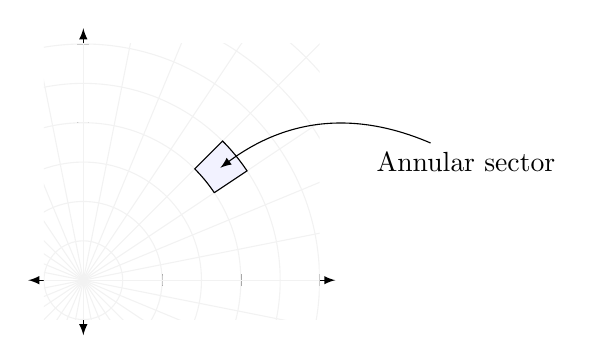
\begin{tikzpicture}[>=latex]

	\begin{scope}
		\clip (-.5,-.5) rectangle (3,3);
		% Draw the lines at multiples of pi/12
		\foreach \ang in {0,...,31} {
		  \draw[gray!10] (0,0) -- (\ang * 180 / 16:4.3);
		}
		
		% Concentric circles and radius labels
		\foreach \s in {0, .5,..., 4} {
		  \draw[gray!10] (0,0) circle (\s);
		}
	\end{scope}

	\draw[fill opacity=0.05, fill=blue] (33.75:2) -- (33.75:2.5) arc (33.75:45:2.5) -- (45:2) arc (45:33.75:2);

			\begin{axis}[
			    anchor=origin,
				name=plot0,
			    set layers=standard,
			    disabledatascaling,
			    xmin=-.25,xmax=1.5,
			    ymin=-.25,ymax=1.5,
			    x=2cm,y=2cm,
			    grid=both,
			    grid style={line width=.1pt, draw=gray!10},
			    %major grid style={line width=.2pt,draw=gray!50},
			    axis lines=middle,
			    minor tick num=0, grid=none,
			    enlargelimits={abs=0.1},
			    axis line style={latex-latex},
			    ticklabel style={font=\tiny,fill=white},
				xticklabels={,,},
				yticklabels={,,},
			    xlabel style={at={(ticklabel* cs:1)},anchor=north west},
			    ylabel style={at={(ticklabel* cs:1)},anchor=south west}
			]
			\end{axis}

		\draw ([xshift=.4cm]plot0.east) node[above right] {Annular sector} edge[bend right, ->] (39.375:2.25);

	\end{tikzpicture}
\end{center}

XXX Figure comparing rectangular chopping and annular sector chopping.

When we compute the exact area of the annular sector between the curves
$\theta=\theta_0$, $\theta=\theta_0+\Delta\theta$, $r=r_0$, and $r=r_0+\Delta r$, 
we get 
\[
	\text{annular sector area} = r_0\Delta r\Delta \theta + \tfrac{1}{2}\Delta\theta(\Delta r)^2.
\]
The first thing to note is that the quantity $r_0$ shows up in the area formula.  
This makes sense, because if you fix two $\theta$ values, the further ``out'' (i.e., the larger
$r_0$ is) you are, the larger the area.  This didn't happen in rectangular coordinates---all the rectangular
sectors had exactly the same area.

Now, just as before, we can write a sum expression for our integral.
\begin{equation}
	\label{EQPOLARSUM}
	\int_{\mathcal D} f\,\d A =\lim_{\Delta r,\Delta \theta\to 0}
	\sum_{r=0,\Delta r,2\Delta r,\ldots,1}\ \ \sum_{\theta=0,\Delta\theta,
	2\Delta\theta, \ldots, 2\pi} \Big(
		r\Delta r\Delta \theta + \tfrac{1}{2}\Delta\theta(\Delta r)^2
	\Big)f(r,\theta)
\end{equation}
However, it isn't clear how to rewrite Equation \eqref{EQPOLARSUM} as an iterated integral
for easy evaluation.

\subsection{Order Analysis}
We can rewrite Equation \eqref{EQPOLARSUM} into one that looks more like a Riemann sum by
doing some \emph{order analysis}\index{order analysis}.  Order analysis allows us to determine
with precision
which parts of an expression become negligible and which parts are non-negligible\footnote{ \emph{Negligible}
is a fancy way of saying ``this can be safely ignored.''}.  Often
times order analysis will show that we can ignore or erase large parts of a formula and still
get the correct answer in the end.


Consider the right hand side of Equation \eqref{EQPOLARSUM}.
\[
	\lim_{\Delta r,\Delta \theta\to 0}
	\sum_{r=0,\Delta r,2\Delta r,\ldots,1}\ \ \sum_{\theta=0,\Delta\theta,
	2\Delta\theta, \ldots, 2\pi} \Big(
		r\Delta r\Delta \theta + \tfrac{1}{2}\Delta\theta(\Delta r)^2
	\Big)f(r,\theta)
\]
In this expression, both $\Delta r$
and $\Delta \theta$ are tending towards $0$ and so 
\[
	r\Delta r\Delta \theta + \tfrac{1}{2}\Delta\theta(\Delta r)^2\to 0.
\]
But, we don't expect the entire limit to go to zero because as $\Delta\theta$ and $\Delta r$
get smaller, each of the two sums get more and more terms.  The outer sum will have roughly
$1/\Delta r$ terms and the inner sum will have roughly $1/\Delta \theta$ terms\footnote{
We say roughly because the number of terms involved is always an integer and the quantities
$1/\Delta r$ and $1/\Delta \theta$ may not be integers.
}.  
Now, $\sum_{i=1}^n K=nK$ if $K$ is a constant.  The inside of our sums are not constant, but if
they were bounded, we could replace them with constants and apply squeeze-theorem arguments to them.
For order analysis, since we are only interested in whether a term
\emph{must} go to zero, we bypass the detailed squeeze theorem arguments 
by just imagining all bounded terms inside our sum are constant and seeing what happens.
To proceed, we first split up
our sum to figure out which parts are negligible.
\[
			\sum_{r=0,\Delta r,2\Delta r,\ldots,1}\ \ \sum_{\theta=0,\Delta\theta,
	2\Delta\theta, \ldots, 2\pi} \Big(
		r\Delta r\Delta \theta + \tfrac{1}{2}\Delta\theta(\Delta r)^2
		\Big)f(r,\theta)
\]
\[
	\phantom{XXXXXXXX}=\sum_{\theta}\sum_{r} r\Delta r\Delta \theta f(r,\theta)
	+ 
		\sum_{\theta}\sum_{r} \tfrac{1}{2}(\Delta r)^2\Delta \theta f(r,\theta)
\]
Doing order analysis on the first part of the sum, we see
\begin{align*}
	\lim_{\Delta r,\Delta\theta\to 0}
	\sum_{\theta}\sum_{r} r\Delta r\Delta \theta f(r,\theta)
	&\sim
	\lim_{\Delta r,\Delta\theta\to 0}
	\frac{1}{\Delta r}\left(\frac{1}{\Delta \theta} \Big(r\Delta r\Delta\theta f(r,\theta)\Big)\right)\\
	&=rf(r,\theta),
\end{align*}
where $\sim$ means \emph{order equivalent}\footnote{ There is a formal theory of
order equivalence and a slew of specialized notations.  We don't need those formalities
right now.}.  Since this term is not order-equivalent to zero, it is non-negligible, and so 
we must keep it.  

Analyzing the other component of the sum tells a different story:
\begin{align*}
	\lim_{\Delta r,\Delta\theta\to 0}
	\sum_{\theta}\sum_{r} \tfrac{1}{2}(\Delta r)^2\Delta \theta f(r,\theta)
	&\sim
	\lim_{\Delta r,\Delta\theta\to 0}
	\frac{1}{\Delta r}\left(\frac{1}{\Delta \theta} \Big(\tfrac{1}{2}(\Delta r)^2\Delta\theta f(r,\theta)\Big)\right)\\
	&=\lim_{\Delta r,\Delta\theta \to 0}\tfrac{1}{2}\Delta rf(r,\theta) = 0,
\end{align*}
and so this part of the sum \emph{is} negligible.  We may therefore conclude,
\[
	\lim_{\Delta r,\Delta \theta\to 0}
	\sum_{r=0,\Delta r,2\Delta r,\ldots,1}\ \ \sum_{\theta=0,\Delta\theta,
	2\Delta\theta, \ldots, 2\pi} \Big(
		r\Delta r\Delta \theta + \tfrac{1}{2}\Delta\theta(\Delta r)^2
	\Big)f(r,\theta)
\]
\[
	=\lim_{\Delta r,\Delta \theta\to 0}
	\sum_{r=0,\Delta r,2\Delta r,\ldots,1}\ \ \sum_{\theta=0,\Delta\theta,
	2\Delta\theta, \ldots, 2\pi} 
		r\Delta r\Delta \theta f(r,\theta),
\]
which is looking a lot more line a Riemann sum that can be converted into an iterated integral.
In fact, if $f$ is a reasonable function (for example, one where Fubini's theorem would hold),
\[
	\lim_{\Delta r,\Delta \theta\to 0}
	\sum_{r=0,\Delta r,2\Delta r,\ldots,1}\ \ \sum_{\theta=0,\Delta\theta,
	2\Delta\theta, \ldots, 2\pi} 
		r\Delta r\Delta \theta f(r,\theta)
		=\int_{\theta=0}^{\theta=2\pi}\int_{r=0}^{r=1}f(r,\theta)r\d r\d \theta.
\]

Order analysis can be very powerful, but we should take note about the assumptions we made.
First off, for the order analysis that we did, we assume $f$ was \emph{bounded} on the region
$\mathcal D$.  We could still do order analysis on an unbounded function, but it would take more 
care\footnote{
	Order analysis on $\sum_{i=1}^n i$ shows that it is order $n^2$, not order $n$.
	This is because the part inside the sum, $i$, is not bounded.
}.  Further, it'd be nice if there were a quicker way to come up with an iterated
integral in various coordinate systems, rather than lugging around Riemann sums
all the time---and there is.

\subsection{The Volume Form}

The \emph{volume form} gives a formal way to rewrite integrals as iterated integrals
with respect to different coordinate systems.  What it really does is give a way
to relate areas or volumes described in a particular coordinate system to ``true''
areas and volumes in Euclidean space---and if your mind is tingling with thoughts
of parameterizations, you're on the right track.


Let's think back to line integrals.  Suppose $\vec p:[a,b]\to\R^n$ is an
arc-length parameterization
of the curve $\mathcal S$. Then, if $f:\R^n\to\R$,
\[
	\int_{\mathcal S} f = \int_{a}^b f\circ \vec p(t) \d t.
\]
However, if $\vec q:[c,d]\to\R^n$ is a non-arc-length parameterization of $\mathcal S$, we have to
use a different formula.  Namely,
\[
	\int_{\mathcal S} f = \int_{c}^d f\circ \vec q(t)\norm{\vec q\,'(t)} \d t.
\]
In this expression, $\norm{\vec q\,'(t)}$ compensates for the fact that as the parameter
$t$ marches on, the arc-length traced out by $\vec q$ is non-uniform.  The volume form\index{volume form} does
the same thing but for parameterizations of multi-dimensional regions.


\begin{definition}[Volume Form]
	Suppose $\mathcal F$ is a coordinate system for $\R^2$ with a relationship
	to rectangular coordinates given by $(x,y)=\vec f(a,b)$.
	The \emph{pre-volume form} associated with $\mathcal F$ at the point $(a,b)$
	is written $\Delta V(a,b)$ and is defined to be the area of
	$\vec f\big([a,a+\Delta a]\times [b,b+\Delta b]\big)$.
	
	The \emph{volume form} associated with $\mathcal F$ at the point $(a,b)$
	is the infinitesimal $\d V(a,b)=V(a,b)\d a\d b$ where $V:\R^2\to\R$ is the 
	unique function satisfying
	\[
		\lim_{\Delta a,\Delta b\to 0} \frac{\Delta V(a,b)}{V(a,b)\Delta a\Delta b}=1.
	\]
\end{definition}
We only wrote down the definition of the volume form for two-dimensional coordinate systems,
but the definition for three and higher dimensions is similar.  To define the
volume form in an $n$-dimensional coordinate system, you take the image
of $n$-dimensional rectangles instead of two-dimensional ones and you replace $\Delta a\Delta b$
with $\Delta x_1\Delta x_2\Delta x_3\cdots\Delta x_n$.

There are a few peculiarities in the definition of the volume form.
First, the word ``infinitesimal'' shows up in the definition.  As of yet,
this has not been a formal term for us.  Further, the volume form has
``$\d a\d b$'' built into it.  These features hark back to the origins
of the volume form.  The term \emph{volume form}
comes from the field of differential geometry, and in differential geometry,
$\d a$ has a unique meaning all by itself and is called a \emph{differential form}.  
Differential forms can be multiplied with each other and added together and the
result still has meaning.
For
us, $\d a$  by itself has no precise
meaning and only appears as a notational book-keeping device in integrals and derivatives.
Of course, the intuitive meaning of $\d a$ is that it is an infinitesimal quantity.
At this point, we won't dive into the details of how and why differential geometry and differential forms
work, but we
will use the language of differential geometry.

\begin{example}
	Compute the volume form for polar coordinates.

	We know that $p:[0,\infty)\times [0,2\pi)\to\R^2$ given 
	by $\vec p(r,\theta)=(r\cos\theta,r\sin\theta)$ converts from polar to rectangular
	coordinates.  Further, we already computed the pre-volume form for polar
	coordinates.  Namely, $\Delta V(r,\theta) = r\Delta r\Delta \theta+\tfrac{1}{2}(\Delta r)^2\Delta \theta$.

	XXX Figure


	To compute the volume form for polar coordinates, we need to find a function $V$ so that
	\begin{align*}
		\lim_{\Delta r,\Delta \theta\to 0}
		\frac{r\Delta r\Delta \theta+\tfrac{1}{2}(\Delta r)^2\Delta \theta}{V(r,\theta)\Delta r\Delta\theta}
		&=\lim_{\Delta r,\Delta \theta\to 0}
		\frac{r}{V(r,\theta)} + \frac{\Delta r}{2V(r,\theta)}\\
		&=\frac{r}{V(r,\theta)} = 1.
	\end{align*}
	There's a clear choice.  Namely, $V(r,\theta)=r$.  Therefore, the volume form for
	polar coordinates is $r\d r\d \theta$.

\end{example}

\subsection{Using the Volume Form}

Once we have gone through the work of finding the volume form for a particular
coordinate system, writing down iterated integrals in that coordinate
system becomes easy---you can just replace ``$\d V$'' with the volume form
and integrate away.

Intuitively the volume form plays the same role that $\norm{\vec q\,'(t)}\d t$ did
in line integrals.  It \emph{compensates} for any stretching or warping that
an alternate coordinate system may do to area.

\begin{example}
	Let $f:\R^2\to\R$ be defined by $f(x,y)=x^2+y^2$ and let $\mathcal D$ be the unit
	disk centered at the origin.  Compute $\int_{\mathcal D} f\,\d V$.

	We've already computed the volume form in polar coordinates.  It is
	$r\d r\d\theta$.  Further, $f$ is easy to describe in polar coordinates,
	since $x^2+y^2=r^2$.  Lastly, in polar coordinates, $\mathcal D$ 
	is the region where $r\in[0,1]$ and $\theta\in[0,2\pi)$.  Therefore,
	\[
		\int_{\mathcal D}f\,\d V =
		\int_{\theta=0}^{\theta=2\pi}\int_{r=0}^{r=1} (r^2)r\d r\d \theta
		=\int_{\theta=0}^{\theta=2\pi}\int_{r=0}^{r=1} r^3\d r\d \theta.
	\]
\end{example}

\begin{example}
	Consider the two-dimensional 
	skewed coordinate system $\mathcal S$.  The $\mathcal S$
	coordinate system uses the variables $a$ and $b$ and relates
	to rectangular coordinates by the equations $x=a+b$ and $y=a-b$.
	Let $f:\R^2\to\R$ be given by the formula $f(a,b)=a+6b$ and let $\mathcal R\subseteq\R^2$
	be the region defined in $\mathcal S$ coordinates by the inequalities
	$1\leq a\leq 2$ and $4\leq b\leq 6$.  Compute $\int_{\mathcal R} f\d V$.

	At present, we have two options.  We could rewrite everything in 
	rectangular coordinates or we could figure out the volume form for $\mathcal S$ 
	coordinates and set our iterated integral up with respect to $\mathcal S$ coordinates.
	Let's do the second way---it sounds more fun.

	Finding the pre-volume form is often the hardest part.  It helps 
	to write down change-of-coordinate functions and draw a picture.
	First off, let $\vec s:\R^2\to\R^2$ be the function that takes points
	written in $\mathcal S$ coordinates and rewrites them in rectangular coordinates.
	From the relationships given above, we see $\vec s(a,b) = (a+b,a-b)$.  Now
	we can draw $[a_0,a_0+\Delta a]\times [b_0,b_0+\Delta b]$ in the $ab$-coordinate
	plane and draw $\vec s([a_0,a_0+\Delta a]\times [b_0,b_0+\Delta b])$ in the
	$xy$-coordinate plane.

	\begin{center}
	\begin{tikzpicture}
		\coordinate (A) at (1,1);
		\coordinate (B) at (3,2);
		\coordinate (D) at ($(B)-(A)$);
		\begin{axis}[
			name=plot1,
		    anchor=origin,
		    disabledatascaling,
		    xmin=-1,xmax=5,
		    ymin=-1,ymax=3,
		    x=1cm,y=1cm,
		    grid=both,
		    grid style={line width=.1pt, draw=gray!10},
		    %major grid style={line width=.2pt,draw=gray!50},
		    axis lines=middle,
		    minor tick num=0,
		    enlargelimits={abs=0.5},
		    axis line style={latex-latex},
			xticklabels={,,},
			yticklabels={,,},
			xlabel={$a$},
			ylabel={$b$},
		    xlabel style={at={(ticklabel* cs:1)},anchor=west},
		    ylabel style={at={(ticklabel* cs:1)},anchor=south}
		]

	\draw[fill=blue,opacity=0.05] (1,1) rectangle (1.8,2.5);	
\addplot[color=myorange, dashed, thick, domain=-3:5] ({1},{x}) node[midway, left,yshift=.5cm] {$a=a_0$};
\addplot[color=myorange, dashed, thick, domain=-3:5] ({1.8},{x}) node[midway, right,yshift=.5cm] {$a=a_0+\Delta a$};
\addplot[color=blue, dashed, thick, domain=-3:5] ({x},{1}) node[midway, below left] {$b=b_0$};
\addplot[color=blue, dashed, thick, domain=-3:5] ({x},{2.5}) node[midway,above left] {$b=b_0+\Delta b$};
	

		\end{axis}

		\draw[] (2.5,3.5) node[above right] {Area in $ab$-plane = $\Delta a\Delta b$};
		\path[thick] (3.5,3.5) edge[bend left, ->] node[] {} (1.5,1.8);


		\begin{axis}[
			%at=(plot1.east),
			at={(7.5,0)},
		    anchor=origin,
		    disabledatascaling,
		    xmin=-1,xmax=5,
		    ymin=-1.4,ymax=3,
		    x=1cm,y=1cm,
		    grid=both,
		    grid style={line width=.1pt, draw=gray!10},
		    %major grid style={line width=.2pt,draw=gray!50},
		    axis lines=middle,
		    minor tick num=0,
		    enlargelimits={abs=0.5},
		    axis line style={latex-latex},
			xticklabels={,,},
			yticklabels={,,},
			xlabel={$x$},
			ylabel={$y$},
		    xlabel style={at={(ticklabel* cs:1)},anchor=west},
		    ylabel style={at={(ticklabel* cs:1)},anchor=south}
		]

	\draw[fill=blue,opacity=0.05] (2,0) -- (3.5,-1.5) -- (4.3,-.7) -- (2.8,.8);	
\addplot[name path=aone, color=myorange, dashed, thick, domain=-3:5] ({1+x},{1-x}) node[near start, left] {$a=a_0$};
\addplot[name path=atwo, color=myorange, dashed, thick, domain=-3:5] ({1.8+x},{1.8-x}) node[near start, right] {$a=a_0+\Delta a$};
\addplot[name path=bone, color=blue, dashed, thick, domain=-3:5] ({x+1},{x-1}) node[at={(0,-2)}, above left] {$b=b_0$};
\addplot[name path=btwo, color=blue, dashed, thick, domain=-3:5] ({x+2.5},{x-2.5}) node[at={(3,-2)}, above left] {$b=b_0+\Delta b$};

	
		\end{axis}	
		\draw[] (2.5+7.5,3.5) node[above right,xshift=-1cm] {Area in $xy$-plane = $V(a_0,b_0)\Delta a\Delta b$};
		\path[thick] (3.5+7.5,3.5) edge[bend left, ->] node[] {} (3+7.5,.2);

	\end{tikzpicture}
	\end{center}

	Conveniently enough, the result is still a rectangle in the $xy$-coordinate plane, so 
	it's area is easy to compute (after finding the lengths of each
	side of the rectangle): $2\Delta a\Delta b$.

	Now, we're looking for a function $V:\R^2\to\R$ so that
	\[
		\lim_{\Delta a,\Delta b\to 0} \frac{2\Delta a\Delta b}{V(a,b)\Delta a\Delta b} = 1,
	\]
	and such a function can be directly guessed.  It's given by $V(a,b)=2$.  Thus,
	the volume form for the $\mathcal S$ coordinate system is $2\d a\d b$.

	Since everything else is already written in terms of the $\mathcal S$ coordinate system,
	we can just write down the iterated integral.
	\begin{align*}
		\int_{\mathcal R} f\,\d V &= \int_{b=4}^{b=6}\int_{a=1}^{a=2} f(a,b)\, 2\d a\d b\\
			&= \int_{b=4}^{b=6}\int_{a=1}^{a=2} 2a+12b\,\d a\d b=126
		.
	\end{align*}
\end{example}

Volume forms are really convenient, but you may be asking: didn't you just stress that
in an expression like $\iint \d a\d b$, the symbols $\d a$ and $\d b$ are not being multiplied
and are just notation?  When we use volume forms aren't we treating $\d a \d b$ like it has meaning
and then working backwards to write down an integral?  This is an astute observation.  Yes,
when we use volume forms, we're assuming that everything will work out as purported.  We won't prove
the details (if you're interested, look in a book on differential geometry), but it is worth noting
that volume forms only exist for \emph{smooth} parameterizations.  That means, every component function
of the parameterization is differentiable in every coordinate.  Most coordinate systems that we
will come across have this property.

When trying to write down an iterated integral in non-rectangular coordinates, computing the volume
form can be the hardest part.  We've been computing volume forms directly from the definition, but
there are several ways that avoid the trouble of finding the pre-volume form.  They include 
the algebra of differential forms and the Jacobian.  We won't discuss the details of these computational
tools here, but it is worth listing the volume forms for some common coordinate systems.

\begin{center}
	\begin{tabular}{c c}
		Coordinate System & Volume Form\\
		\hline
		Rectangular Coordinates in $\R^2$ & $\d x\d y$\\
		Polar Coordinates & $r\d r\d \theta$\\
		Rectangular Coordinates in $\R^3$ & $\d x\d y\d z$\\
		Cylindrical Coordinates & $r\d r\d \theta\d z$\\
		Spherical Coordinates & $r^2\sin\phi\d r\d \phi\d \theta$
	\end{tabular}
\end{center}

\subsection{The Chain Rule for Volume Forms}
Suppose $\vec p:\R^2\to\R^2$ is a parameterization.  We can think of $\vec p$ as a function
that takes points in one coordinate system and outputs points in rectangular coordinates.
Call the coordinate system that $\vec p$ inputs the $\mathcal P$ coordinate system with variables
$\alpha$ and $\beta$.  Now, there is some volume form associated with the $\mathcal P$ coordinate
system and it takes the form $V_{\vec p}(\alpha,\beta)\d\alpha \d\beta$.  We interpret $V_{\vec p}(\alpha,\beta)$
as the amount that $\vec p$ stretches or shrinks volume by at the point $(\alpha,\beta)$ (in $\mathcal P$ coordinates).

Now, suppose $\vec q:\R^2\to\R^2$ is another parameterization.  Similarly to $\vec p$, associate
$\vec q$ with the $\mathcal Q$ coordinate system with variables $\gamma$ and $\delta$.  Let
$V_{\vec q}(\gamma,\delta)\d\gamma\d\delta$ be the volume form for $\mathcal Q$ coordinates.

Now, $\vec p$ and $\vec q$ relate to coordinate systems, but they are really just parameterizations with domain
$\R^2$ and range $\R^2$.  So, $\vec s=\vec q\circ \vec p$ is another parameterization.
Associate it with the $\mathcal S$ coordinate system with the variables $a$ and $b$.  Can we write the volume
form for the $\mathcal S$ coordinate system in terms of the volume form for $\mathcal P$ and
$\mathcal Q$ coordinates?

Yes, we can!  The process is fairly straightforward.  We know $V_{\vec p}(\alpha,\beta)$ is how
much $\vec p$ changes area by at the point $(\alpha,\beta)$ and we know $V_{\vec q}(\gamma,\delta)$
is how $\vec q$ changes area at the point $(\gamma,\delta)$.  Further, considering the composition
$\vec s=\vec q\circ \vec p$, we could interpret $\vec p$ as inputing $\vec P$ coordinates and then
outputting $\vec Q$ coordinates, which then get taken by $\vec q$ and finally converted to rectangular coordinates.
Thus, at the point $(\alpha,\beta)$, area first gets changed by $V_{\vec p}(\alpha,\beta)$
and then at the point $\vec p(\alpha,\beta)$, area gets changed by $V_{\vec q}\circ \vec p(\alpha,\beta)$.
Change in area is multiplicative, so
\begin{equation}
	\label{EQVOLFORMCHAINRULE}
	V_{\vec s}(\alpha,\beta) = V_{\vec p}(\alpha,\beta)\Big(V_{\vec q}\circ \vec p(\alpha,\beta)\Big).
\end{equation}
Does that look a little like the chain rule?

Let's try this again in one dimension.  Let $f:\R\to\R$ and $g:\R\to\R$ both be parameterizations.
In one dimension the limit involved in finding a volume form turns out to be equivalent to taking
a derivative (go ahead, compute the one-dimension volume form of a few of your favorite functions!).
Therefore,
\[
	V_{f}(a) = f'(a)\qquad\text{and}\qquad V_{g}(b) = g'(b).
\]
Let $h=g\circ f$.  Expanding with Equation \eqref{EQVOLFORMCHAINRULE}, we get
\[
	h'(a) = V_{h}(a) = V_f(a)\Big(V_g\circ f(a)\Big) = f'(a)\Big(g'\circ f(a)\Big),
\]
which is exactly what the chain rule says!  This is no coincidence. Equation
\eqref{EQVOLFORMCHAINRULE} really is the chain rule in disguise\footnote{ 
Hold the phone!  There's something strange going on.  The derivative
of a function can take negative values but by definition a volume form must take only
positive values.  So, on the surface $w'=V_{w}$ can only hold for special parameterizations
$w:\R\to\R$.  This is true, and this is all fixed in the land of differential forms
where volumes and areas are allowed to be \emph{signed}.}.  

%While we're still in the mood to look at Equation \eqref{EQVOLFORMCHAINRULE}, let's
%make one more observation.  We could interpret the symbol ``$V$'' as an operator
%that inputs a function and outputs a new function.  Namely,
%if $\vec w:\R^n\to\R^n$, then $V_{\vec w}:\R^n\to\R$ is a function associated
%with $\vec w$.  Let's choose a more evocative notation for ``$V$''.  Define and alternate notation
%for ``$V$'' by
%\[
%	V_{\vec w}(\vec x) = \frac{\d \vec w}{\d \vec x}.
%\]
%In this notation, Equation \eqref{EQVOLFORMCHAINRULE} says
%\[
%	\frac{\d \vec s}{\d \vec x} = \frac{\d\vec p}{\d \vec x}\,\frac{\d\vec q}{\d \vec p}.
%\]
%Now this really looks like the chain rule! At this point, using a notation that looks like
%derivative notation is mostly whimsy---when $\vec w:\R^n\to\R^n$ and $n>1$,
%we don't even know what the derivative of $\vec w$ should mean---but 
%in the field of differential geometry, such notation can be justified.
%
%
%Enough whimsy.  
Let's use the chain rule for volume forms to solve a problem.
\begin{example}
	XXX Finish.  Maybe an isometric rotation and a stretching of some sort?
\end{example}

\begin{exercises}
\end{exercises}

\section{Surface Integrals}
We will now turn our attention to integrals over non-flat regions.  Suppose
we wanted to find the average temperature of the surface of a perfectly
spherical earth.  Conceptually, we can compute this with a Riemann sum
just like before.  We chop the surface of the earth up into little regions
and find the temperature in each region.  We then compute
\[
	\text{average temp}\quad\approx\quad\frac{1}{\text{total surface area}} \sum_{\text{sectors}}
	(\text{temp at sector})(\text{area of sector}),
\]
with equality after we take a limit as the sector size tends towards zero.  

\begin{example}
	\label{EXSURFACEAREABYDEF}
	Let $\mathcal S\subseteq \R^3$ be the unit sphere centered at the origin,
	and consider the parameterization $\vec s:[0,2\pi)\times[0,\pi]\to\mathcal S$ of $\mathcal S$ given
	by
	\[
		\vec s(\theta,\phi) = \matc{\sin\phi\cos\theta\\\sin\phi\sin\theta\\\cos\phi}.
	\]
	We wish to compute the average value of $T:\mathcal S\to\R$ over the surface $\mathcal S$.

	The parameterization $\vec s$ gives us a natural way to chop $\mathcal S$ up into tiny pieces.
	In particular, if $\Delta \theta$ and $\Delta \phi$ are tiny then $\vec s\big([\theta_0,\theta_0+\Delta
	\theta]\times[\phi_0,\phi_0+\Delta\phi]\big)\subseteq\mathcal S$ will be a tiny sector
	of $\mathcal S$.

	XXX Figure

	The exact area of this sector turns out to be $\big(\cos\phi_0-\cos(\phi_0+\Delta\phi)\big)\Delta\theta$.
	The total surface area of $\mathcal S$ is $4\pi$ and so we have
	\[
		\text{average of }T\quad=\quad \frac{1}{4\pi}\  \lim_{\Delta\theta,\Delta\phi\to0}
		\sum_{\theta_i}\sum_{\phi_i} T\circ \vec s(\theta_i,\phi_i)\Big(\cos\phi_i-\cos(\phi_i+\Delta\phi)\Big)\Delta\theta,
	\]
	where the sums are taken over $\theta_i=0,\Delta\theta,2\Delta\theta,\ldots,2\pi$ and
	$\phi_i=0,\Delta\phi,2\Delta\phi,\ldots,\pi$.

	Evaluating that Riemann sum looks challenging, but we can use the idea of volume
	forms to rewrite it as an iterated integral.  Notice
	\[
		\lim_{\Delta\theta,\Delta\phi\to0} \frac{\big(\cos\phi-\cos(\phi+\Delta\phi)\big)\Delta \theta}
		{\Delta \phi\Delta\theta}
		=\,-\lim_{\Delta\theta,\Delta\phi\to0} \frac{\cos(\phi+\Delta\phi)-\cos\phi}
		{\Delta \phi} = \sin\phi,
	\]
	since the expression in the middle is just the derivative of cosine in disguise.  Now,
	we can view $T\circ \vec s$ as a function from $\R^2\to\R$ being integrated in a different
	coordinate system.  And, we just computed the volume form of that different coordinate
	system to be $\sin\phi\d\phi\d\theta$.  Therefore,
	\[
		\text{average of }T\quad=\quad\frac{1}{4\pi}\int_{\theta=0}^{\theta=2\pi}\int_{\phi=0}^{\phi=\pi}
		T\circ \vec s(\theta,\phi)\sin\phi\d\phi\d\theta.
	\]
	Given a formula for $T$, we now have a much better chance of being able to evaluate its average!
\end{example}

The reasoning used in Example \ref{EXSURFACEAREABYDEF} closely follows the reasoning
used for integrating functions over flat regions, and we would be justified in extending our integral
notation.  If $\mathcal S\subseteq\R^3$ is a surface and $f:\mathcal S\to\R$ is a function,
then
\[
	\int_{\mathcal S} f  = \int_{\mathcal S} f\,\d A
\]
is defined to be result of chopping up $\mathcal S$ into tiny sectors, summing up the
area of each sector multiplied by the value of $f$ on that sector, and then taking the limit as
the size of each sector goes to zero.  Just like before, since we don't explicitly define the way
that $\mathcal S$ must be chopped up into sectors and we don't define the order in which we
should sum the sectors, the expression $\int_{\mathcal S}f$ is only defined if the way we chop
and the order we sum doesn't matter.  Again, if $f$ and $\mathcal S$ are nice (for example, $\mathcal S$
has a tangent plane at every point and $f$ satisfies the conditions of Fubini's theorem), then
$\int_{\mathcal S} f$ is defined.  Most functions and surfaces we will encounter will be nice.

Another thing to notice about Example \ref{EXSURFACEAREABYDEF} is that doing the
computation was somewhat difficult.
For starters, how could we find the sector area if we weren't given an explicit formula for it?
This is as difficult, if not more difficult, than finding the pre-volume form\footnote{
At this point, we don't actually have a definition of the ``surface area'' of a curved surface, 
so how could we compute the area of a sector?}.  Like we did with volume forms, we will leverage
our intuition and leave it to other mathematicians to verify the details.

\subsection{Approximating Surfaces}

Suppose $\mathcal S\subset \R^3$ and that $\vec s\in\mathcal S$.  Let $\mathcal P_{\vec s}$ be the
tangent plane to $\mathcal S$ at the point $\vec s$.  There are many ways we could write down
a formula for $\mathcal P_{\vec s}$, but if we were given a parameterization for $\mathcal S$,
there would be a particularly direct way to describe $\mathcal P_{\vec s}$ in vector form.

\begin{definition}[Canonical Representation of the Tangent Plane]
	Given a surface $\mathcal S\subseteq\R^3$ parameterized by $\vec p:\R^2\to\mathcal S$,
	the \emph{canonical representation} of the tangent plane to $\mathcal S$
	relative to the parameterization $\vec p$
	at the point $\vec p(a,b)\in\mathcal S$ is given by the first-order
	(affine) approximation to $\vec p$ at $(a,b)$.  In vector form, this representation
	is
	\[
		\vec x = t \frac{\partial \vec p}{\partial a}(a,b) + s\frac{\partial \vec p}{\partial b}(a,b)
		+\vec p(a,b).
	\]
\end{definition}

There are two ways to unpack the canonical representation of a tangent plane.
Let $\mathcal S\subseteq\R^3$ be parameterized by $\vec p:\R^2\to\mathcal S$ as before
and let $\vec s\in\mathcal S$.  Further, suppose that $\vec p(a,b)=\vec s$.  Now,
to write down a formula for the tangent plane $\mathcal P_{\vec s}$, all we need is to
find two vectors, $\vec d_1$ and $\vec d_2$, that are tangent to $\mathcal S$ at the point $\vec s$.
Then, we can describe $\mathcal P_{\vec s}$ in vector form by
\[
	\vec x=t\vec d_1+s\vec d_2+\vec s.
\]
Further, the curve traced out by $\vec p(t,b)$ as $t$ varies and $b$ is held constant is
contained in $\mathcal S$ and passes through $\vec s$ exactly when $t=a$.  Therefore, we can
find a tangent vector to $\mathcal S$ at $\vec s$ by finding a velocity vector for this curve.
\[
	\frac{\d}{\d t} \vec p(t,b)\Big|_{t=a} = \frac{\partial \vec p}{\partial a}(a,b).
\]
Similarly, we can find a second tangent vector by considering the curve traced out by $\vec p(a,t)$
as $t$ varies and $a$ is held constant.  This gives us a tangent vector of
\[
	\frac{\d}{\d t} \vec p(a,t)\Big|_{t=b} = \frac{\partial \vec p}{\partial b}(a,b).
\]

XXX Figure

For all reasonable parameterizations, $\frac{\partial \vec p}{\partial a}(a,b)$ and $\frac{\partial \vec p}{\partial b}(a,b)$
will point in different directions, and so we may represent $\mathcal P_{\vec s}$ in vector form as
	\begin{align*}
		\vec x &= t \frac{\partial \vec p}{\partial a}(a,b) + s\frac{\partial \vec p}{\partial b}(a,b)
		+\vec s\\
		&= t \frac{\partial \vec p}{\partial a}(a,b) + s\frac{\partial \vec p}{\partial b}(a,b)
		+\vec p(a,b).
	\end{align*}
This is the \emph{canonical} way to write down a tangent plane if you are given a parameterization.


There's another way to view the canonical representation of the tangent plane with respect to $\vec p$,
and that is as a first-order approximation.  Recall that to find the first-order approximation
of a function $\vec p:\R^2\to\R^3$, you first find the first-order approximations of each of $\vec p$'s
component functions.  These component approximations become the component functions
of the first order approximation to $\vec p$.  When all is said and done, we arrive at the following
formula for $\vec L_{\vec p}$, the first-order approximation of $\vec p$ at the point $(a,b)$.
\[
	\vec L_{\vec p}(t,s) = t \frac{\partial \vec p}{\partial a}(a,b) + s\frac{\partial \vec p}{\partial b}(a,b)
		+\vec p(a,b)
\]

Let $\vec L_{\vec p}:\R^2\to\R^3$ be the canonical representation of the tangent plane to $\mathcal S$,
relative to $\vec p$, at the point $\vec p(a,b)$.  Since $\vec L_{\vec p}$ is a first-order
approximation to $\vec p$, we know that if $(t,s)$ is close to $(a,b)$, then
\[
	\vec L_{\vec p}(t,s)\approx \vec p(t,s).
\]
It's now not so far fetched to to believe
\[
	\text{area of }\vec L_{\vec p}([a,a+\Delta a]\times [b,b+\Delta b]) \approx
	\text{area of }\vec p([a,a+\Delta a]\times [b,b+\Delta b]).
\]
That is, the area of the tiny sector in $\mathcal S$ close to the point $\vec p(a,b)$
is approximately equal to the area of the corresponding
tiny sector on the tangent plane to $\mathcal S$ at the point $\vec p(a,b)$.

XXX Figure

In fact, if $\vec p$ is differentiable, we have
\[
	\lim_{\Delta a,\Delta b\to0} \frac{\text{area of }\vec L_{\vec p}([a,a+\Delta a]\times [b,b+\Delta b])}{\Delta a\Delta b}
	=
	\lim_{\Delta a,\Delta b\to0} \frac{\text{area of }\vec p([a,a+\Delta a]\times [b,b+\Delta b])}{\Delta a\Delta b},
\]
which is exactly what we need to compute a volume form!

\begin{exercises}
\end{exercises}
